\documentclass[12pt,oneside,english,reqno]{amsbook}
\usepackage[utf8]{inputenc}
 \author{Vadim Yerokhin}
\date{\today}
 

 \renewcommand{\familydefault}{\rmdefault}
%\usepackage[T1]{fontenc}

\usepackage{geometry}
\geometry{verbose,tmargin=1in,bmargin=1in,lmargin=1in,rmargin=1in}
\usepackage{mathrsfs}
\usepackage{url}

\usepackage{amstext}
\usepackage{stmaryrd}
\usepackage{setspace}
\doublespacing

\makeatletter

%%%%%%%%%%%%%%%%%%%%%%%%%%%%%% LyX specific LaTeX commands.
%% A simple dot to overcome graphicx limitations
\newcommand{\lyxdot}{.}


%%%%%%%%%%%%%%%%%%%%%%%%%%%%%% Textclass specific LaTeX commands.
\numberwithin{section}{chapter}
\numberwithin{equation}{section}
\numberwithin{figure}{section}

\makeatother

\usepackage{babel}

\usepackage{bm, graphicx, amsmath}
\usepackage{bbm}

 \newcommand{\abs}[1]{\left|{#1}\right|}
 \newcommand{\av}[1]{\left\langle #1 \right\rangle}
 
  \newcommand{\br}[1]{\langle #1|}
  \newcommand{\ke}[1]{|#1\rangle}
  \newcommand{\bk}[2]{\langle #1|#2\rangle}
  \newcommand{\kb}[2]{\ke{#1}\br{#2}}
  \newcommand{\var}[2]{\langle #1,#2\rangle} 
  
  \newcommand{\al}[1]{^{(#1)}}
  \newcommand{\da}{^\dagger} 
  
  \newcommand{\pt}[1]{\left( #1 \right)}
  \newcommand{\pq}[1]{\left[ #1 \right]}
  \newcommand{\pg}[1]{\left\{ #1 \right\}} 
  
  \newcommand{\lpt}[1]{\left( #1 \right.}
  \newcommand{\lpq}[1]{\left[ #1 \right.]}
  \newcommand{\lpg}[1]{\left\{ #1 \right.}
  \newcommand{\rpt}[1]{\left. #1 \right)}
  \newcommand{\rpq}[1]{\left. #1 \right]}
  \newcommand{\rpg}[1]{\left. #1 \right\}} 


\newcommand{\td}[1]{\widetilde{#1}}
\begin{document}

\global\long\def\sandwich#1#2#3{ \left\langle #1\left|#2\right|#3\right\rangle }
\global\long\def\ket#1{\left|#1\right>}
\global\long\def\braket#1#2{\left\langle #1\mid#2\right\rangle }
\global\long\def\bra#1{\left\langle #1\right|}
\global\long\def\indep{\perp\!\!\!\perp}


\title{Dissertation}
\maketitle
\tableofcontents
 
\part{Introduction}
\chapter{Hello}

\section{Introduction}

Interacting with the universe on a fundamental level involves quantum mechanical principles different than those
of 

realm of new possibilitites

*vomit*

\subsection{Why Measurement Theory?}
Classical bits versus quantum bits: instead of just a 0 or 1, quantum bits can maintain a superposition state

The probabalistic nature of detection: only orthogonal states can be discriminated perfectly

Quantum Computing

Quantum Communication
\subsection{State Representation and the Density Matrix }
A density matrix is a generalized state that is a statistical collection of pure states defined by four properties:

1. $\rho  = \sum_i \eta_i \kb{\psi_ i}{\psi_i}$ where $\sum \eta_i = 1$


2. It is Hermitian 

3.  $Tr \rho = 1$

4. $\br {\phi_i} \rho \ke {\phi_i} \geq 0$
{Measurement Operators}

Measurements are a decomposition of the identity in terms of positive semi-definite matrices.

    A measurement can be either a projector or a generalized measurement.  In the latter case it must fulfill only 2 properties:

           1.  $\sum \Pi_i = 1$


	2. They are Hermitian.  This corresponds to real eigenvalues (measurement outcomes).



{Expectation Values as Traces}
Since non-orthogonal states cannot be discriminated perfectly, we can speak of the probability of a given outcome:




	$\av {\Pi_i} = \sum_j \eta_j \br {\psi_j} \Pi_i \ke {\psi_j} = Tr(\Pi_i \rho)$


\subsection{The Measurement Process}

\chapter{Pure State Discrimination}


\section{Minimum Error Measurements}
The first measurement strategy was Minimum Error Discrimination.

	Two orthogonal projectors, each clicks for a state.

	There is a success rate and an error rate if the states are not orthogonal.

\[ P_s =\eta_1 Tr(\rho_1 \Pi_1) + \eta_2Tr(\rho_2 \Pi_2)\]
\[ P_e = \eta_2 Tr(\rho_2 \Pi_1) +\eta_1 Tr(\rho_1 \Pi_2)\]

	The minimum error rate for pure states is achieved by the Helstrom bound.

\[P_E = \frac{1}{2}(1- \sqrt{1-4 \eta_1 \eta_2 \kb{\psi_1}{\psi_2}})\]

\section{Unambiguous Discrimination}
Make the measurement operators orthogonal to the state that we don't want to measure.

	Since they are no longer orthogonal they don't sum to the identity. A third, inconclusive outcome is necessary.

	The detector corresponding to the inconclusive outcome we call $\Pi_0$

	The failure probability we call Q:

\[Q =  \eta_1 Tr(\rho_1 \Pi_0) +\eta_2  Tr(\rho_2 \Pi_0) = Tr(\rho \Pi_0)\]

$ Q_0 = 2 \sqrt{\eta_1\eta_2} cos \theta$  is the failure rate that corresponds to the best measurement.

{Unambiguous State Discrimination Graph}

\section{Intermediate Discrimination}

\subsection{Transformation Solution}
We review the original problem in a single two-dimensional Hilbert space, and the solution that  involves a transformation that eliminates the failure operator from the discrimination problem.  We are given two pure states $\rho_1= \ke \psi_1 \br {\psi_1}$ and $\rho_2 = \ke \psi_2 \br{\psi_2}$ with a-priori probabilities $\eta_1$ and $\eta_2$ respectively.  These two probabilities add to one:  $\eta_1 +\eta_2 = 1$. We wish to optimize the success rate  $P_s = \eta_1tr[\Pi_1 \rho_1] + \eta_2 tr[\Pi_2 \rho_2]$ for a fixed failure rate $Q = tr[\Pi_0(\eta_1 \rho_1 + \eta_2 \rho_2)]$ where the measurement operators are the $\Pi_i$ that span the Hilbert space: $\Pi_1 + \Pi_2 + \Pi_0 = I$.  The transformation we implement is
 \begin{equation}
\Omega ^{-1/2}[\Pi_1 + \Pi_2] \Omega^{-1/2} = I,
\end{equation}
where $\Omega = I - \Pi_0$.

Calling the transformed operators $\widetilde \Pi_i$ for $i= 1,2$, we can find the corresponding transformed density matrices $\widetilde \rho_i$ and a-priori probabilities $
\widetilde \eta_i$ to make this a new ME problem that can be readily solved. The minimized error probability as a function of the failure rate is
\begin{equation} P_e = \frac{1}{2} (1 - Q -\sqrt{(1-Q)^2 - (Q-Q_0)^2})\end{equation}
for $Q \leq Q_0 = 2 \sqrt{\eta_1\eta_2} \cos \theta$ where $Q_0$ is the maximum failure rate allowed in the optimization scheme and it corresponds to the best measurement in the UD case.  We will provide an in-depth description of this solution as it pertains to our problem in the next section.


%%%%%%%%%%%%%%%%%%%%%%%%%%%%%%%%%%%%%%%%%%%%%%%%%%%%%%%%%%EX%%%%%%%%%%%%%%%%%%%%%%%%%%%%%%%%%%%%%%%%%%%%%%%%%%%%%%%%%%%%% 
%%%%%%%%%%%%%%%%%%%%%%%%%%%%%%%%%%%%%%%%%%%%%%%%%%%%%%%%%%%%%%%%%%%%%%%%%%%%%%%%%%%%%%
%%%%%%%%%%%%%%%%%%%%%%%%%%%%%%%%%%%%%%%%%%%%%%%%%%%%%%%%%%EX%%%%%%%%%%%%%%%%%%%%%%%%%%%%%%%%%%%%%%%%%%%%%%%%%%%%%%%%%%%%% 
%%%%%%%%%%%%%%%%%%%%%%%%%%%%%%%%%%%%%%%%%%%%%%%%%%%%%%%%%%%%%%%%%%%%%%%%%%%%%%%%%%%%%%

%%%%%%%%%%%%%%%%%%%%%%%%%%%%%%%%%%%%%%%%%%%%%%%%%%%%%%%%%%EX%%%%%%%%%%%%%%%%%%%%%%%%%%%%%%%%%%%%%%%%%%%%%%%%%%%%%%%%%%%%% 
%%%%%%%%%%%%%%%%%%%%%%%%%%%%%%%%%%%%%%%%%%%%%%%%%%%%%%%%%%%%%%%%%%%%%%%%%%%%%%%%%%%%%%
%%%%%%%%%%%%%%%%%%%%%%%%%%%%%%%%%%%%%%%%%%%%%%%%%%%%%%%%%%EX%%%%%%%%%%%%%%%%%%%%%%%%%%%%%%%%%%%%%%%%%%%%%%%%%%%%%%%%%%%%% 
%%%%%%%%%%%%%%%%%%%%%%%%%%%%%%%%%%%%%%%%%%%%%%%%%%%%%%%%%%%%%%%%%%%%%%%%%%%%%%%%%%%%%%


\part{Interpolative Discrimination of Mixed States}

%%%%%%%%%%%%%%%%%%%%%%%%%%%%%%%%%%%%%%%%%%%%%%%%%%%%%%%%%%EX%%%%%%%%%%%%%%%%%%%%%%%%%%%%%%%%%%%%%%%%%%%%%%%%%%%%%%%%%%%%% 
%%%%%%%%%%%%%%%%%%%%%%%%%%%%%%%%%%%%%%%%%%%%%%%%%%%%%%%%%%%%%%%%%%%%%%%%%%%%%%%%%%%%%%
%%%%%%%%%%%%%%%%%%%%%%%%%%%%%%%%%%%%%%%%%%%%%%%%%%%%%%%%%%EX%%%%%%%%%%%%%%%%%%%%%%%%%%%%%%%%%%%%%%%%%%%%%%%%%%%%%%%%%%%%% 
%%%%%%%%%%%%%%%%%%%%%%%%%%%%%%%%%%%%%%%%%%%%%%%%%%%%%%%%%%%%%%%%%%%%%%%%%%%%%%%%%%%%%%

\chapter{Mixed State Discrimination in Subspaces}

%%%%%%%%%%%%%%%%%%%%%%%%%%%%%%%%%%%%%%%%%%%%%%%%%%%%%%%%EX%%%%%%%%%%%%%%%%%%%%%%%%%%%%%%%%%%%%%%%%%%%%%%%%%%%%%%%%%%%%% 
%%%%%%%%%%%%%%%%%%%%%%%%%%%%%%%%%%%%%%%%%%%%%%%%%%%%%%%%%%%%%%%%%%%%%%%%%%%%%%%%%%%%%%

\section{Jordan Basis Structure}
To discuss the more general case of higher-dimensional input states we consider a Jordan Basis structure.
Two states are now to be discriminated with a-priori probabilities $\eta_1 , \eta_2$ such that $\rho_1 = \sum r_i \vert r_i \rangle \langle r_i \vert $ and $\rho_2 = \sum s_i \vert s_i \rangle \langle s_i \vert$ with $ \langle r_i \vert s_j \rangle = \delta_{ij} \cos \theta_i$. In each 2d subspace i there lie an $\vert r_i \rangle$ and  $\vert s_i \rangle$ with a-priori probabilities now
$\eta_{1,i} = \eta_1 r_i$ and $\eta_{2,i} = \eta_2 s_i$.  This structure can be physically interpreted as the transmission of two input states over several fiber optic cables. Each cable contains two degrees of freedom, that could be horizontal and vertical polarization.

The generalization to multiple subspaces is straightforward at first  so we begin with the two subspaces example.

Here our density matrices are in four dimensions that can be described as two tensor product spaces:
\begin{eqnarray}
 \rho_1 &=& r_1 \vert r_1 \rangle \langle r_1 \vert  + r_2 \vert r_2 \rangle \langle r_2 \vert \\
 \rho_2 &=& s_1 \vert s_1 \rangle \langle s_1 \vert  + s_2 \vert s_2 \rangle \langle s_2 \vert. \nonumber\end{eqnarray}
These mixed states are shown in Fig. 1.


Defining our measurement operators for the first subspace as
\begin{equation} \widetilde \Pi_{1,1} + \widetilde \Pi_{2,1} = I_1,\end{equation}
where $I_1$ is the identity matrix of the first subspace.  We define the failure rate for the first subspace as $Q_1 = \xi_1 \ke 0_{11} \br 0 $,which in terms of a measurement probability is also
\begin{equation} Q_1 = \xi_1 [ \eta_{1,1} \cos^2 \phi_1 + \eta_{2,1} \cos^2 (\theta_1 - \phi_1)],\end{equation}
where $\theta_1 $ is the overlap angle between the two states in subspace 1, and $\phi_1$ is the angle $\ke {r_1}$ makes with respect to $\vert 0 \rangle_1$.  The error rate in that subspace is
\begin{equation}P_{e,1} = \eta_{1,1} \langle r_1 \vert \Pi_2 \vert r_1 \rangle + \eta_{2,1} \langle s_1 \vert \Pi_1 \vert s_1 \rangle. \end{equation}
For our simplification trick to work we introduce the normalized state vector \begin{equation} \vert \widetilde{r_1} \rangle  = \frac{ \Omega^{1/2} \vert r_1 \rangle}{\sqrt{\langle r_1 \vert \Omega \vert r_1 \rangle}} \end{equation}
and normalized coefficients
\begin{equation} \widetilde{\eta_{1,1}} = \frac{\eta_{1,1} \langle r_1 \vert \Omega \vert r_1 \rangle}{\eta_{1,1} \langle r_1 \vert \Omega \vert r_1 \rangle + \eta_{2,1} \langle s_1 \vert \Omega \vert s_1 \rangle}\end{equation}
to get 
\[P_{e,1}= \]
\[ [\eta_{1.1} \langle r_1 \vert \Omega \vert r_1 \rangle + \eta_{2,1}\langle s_1 \vert \Omega \vert s_1 \rangle](\widetilde{\eta_{1,1}}\langle\widetilde{r_1} \vert \widetilde{\Pi_2} \vert \widetilde{r_1} \rangle + \widetilde{\eta_{2,1}} \langle \widetilde{s_1} \vert \widetilde{\Pi_1} \vert \widetilde{s_1}\rangle ).\]

We notice that the expression in the ( ) with all tildes contains a pure state minimum error problem, while with the notation $ \eta_{1,1} +\eta_{2,1} = \omega_1$ the left hand set of [ ]  can be reworked into $\omega_1 - Q_1 $ to rewrite the error rate as
\[ P_{e,1}= \frac{1}{2} [\omega_1 - Q_1] (1- \sqrt{1 - 4 \widetilde{\eta_{1,1}} \widetilde{\eta_{2,1}} \vert \langle \widetilde{r_1} \vert \widetilde{s_1} \rangle \vert ^2 }). \]
If we substitute and simplify we find this equals to
\[=\frac{1}{2} ( \omega_1 - Q_1 - \sqrt{ ( \omega_1 - Q_1)^2 -(Q_{0,1} - Q_1 \sin 2 \phi )^2}),\]
where we used the notation $Q_{0,1} = 2 \sqrt{\eta_{1,1}\eta_{2,1}} \cos \theta_1$ and 
 $ \sin \phi = \frac{ \sqrt {\eta_{2,1}} \cos (\theta_1 - \phi_1)}{\sqrt{ \eta_{1,1} \cos^2 (\phi_1)+ \eta_{2,1} \cos^2 (\theta_1 - \phi_1)}}$.  Minimization of the error rate as a function of $\phi_1$ tells us to set $\phi_1 =\frac{\pi}{4}$ so finally
\begin{equation}P_{e,1} = \frac{1}{2} ( \omega_1 - Q_1 - \sqrt{ ( \omega_1 - Q_1)^2 -(Q_{0,1} - Q_1 )^2}).\end{equation}

This result agrees with the single subspace limit and is simply the optimized solution for that subspace alone. We can derive a similar result for the other subspace, so we can consider an optimal distribution of failure among the two subspaces.  However, we want to treat this distribution problem for n subspaces so we first generalize our preceding solution to 2n dimensions.


Recognizing that the likelihood of finding a particle in a subspace isn't 1, we want to normalize our problem so that we can solve it like the 2d case where we had $P_e+ P_s+ Q= 1.$ Instead, in our problem we have $P_{e,i} + P_{s,i} + Q_i = \eta_{1,i} + \eta_{2,i} = \omega_i$ where $P_{s,i}$ and $Q_i$ are the success and the failure probabilities in that subspace.  Since our measurements span the Hilbert space of this subspace, the total probability of a particle being measured therein we call $\omega_i$, or the weight of that subspace.

We can define weighted result probabilities
\begin{equation} \bar{P_{e,i}} +\bar{P_{s,i}} + \bar{Q_i} = 1 \end{equation}
with $ \bar{\bullet} = \frac{\bullet}{\omega_i} $. We can define new constants $\bar{\eta_{1,i}} $ and $ \bar{\eta_{2,i}}$ that still sum 1, so that the states and measurements in (3.8) don't change.  Now it is straightforward to apply the 2d solution to each subspace, where our error rate becomes
\[\bar{P_{e,i}} = \frac{1}{2}( 1-\bar{Q_i} - \sqrt{(1-\bar{Q_i})^2 - (\bar{Q_{0,i}} -\bar{ Q_i})^2}),\]
where $\bar{Q_{0,i}} = 2 \sqrt{\bar{\eta_{1,i}}\bar{\eta_{2,i}}}\cos\theta_i.$
If we remove the bars, this becomes the generaized version of the solution we derived for one subspace in (3.7):
\begin{equation}P_{e,i}= \frac{1}{2}( \omega_i-Q_i - \sqrt{(\omega_i-Q_i)^2 - (Q_{0,i} - Q_i)^2}).\end{equation}

%%%%%%%%%%%%%%%%%%%%%%%%%%%%%%%%%%%%%%%%%%%%%%%%%%%%%%%%%%EX%%%%%%%%%%%%%%%%%%%%%%%%%%%%%%%%%%%%%%%%%%%%%%%%%%%%%%%%%%%%% 
%%%%%%%%%%%%%%%%%%%%%%%%%%%%%%%%%%%%%%%%%%%%%%%%%%%%%%%%%%%%%%%%%%%%%%%%%%%%%%%%%%%%%%
\section{Subspaces formalism}

To discuss the more general case of higher-dimensional input states we consider a Jordan Basis structure.
Two states are now to be discriminated with a-priori probabilities $\eta_1 , \eta_2$ such that $\rho_1 = \sum r_i \vert r_i \rangle \langle r_i \vert $ and $\rho_2 = \sum s_i \vert s_i \rangle \langle s_i \vert$ with $ \langle r_i \vert s_j \rangle = \delta_{ij} \cos \theta_i$. In each 2d subspace i there lie an $\vert r_i \rangle$ and  $\vert s_i \rangle$ with a-priori probabilities now
$\eta_{1,i} = \eta_1 r_i$ and $\eta_{2,i} = \eta_2 s_i$.  This structure can be physically interpreted as the transmission of two input states over several fiber optic cables. Each cable contains two degrees of freedom, that could be horizontal and vertical polarization.

The generalization to multiple subspaces is straightforward at first  so we begin with the two subspaces example.  

%%%%%%%%%%%%%%%%%%%%%%%%%%%%%%%%%%%%%%%%%%%%%%%%%%%%%%%%%%%%%%%%%%%%%%%%%%%%%%%%%%%%%%%%%%%%%%%%%%%%%%%%%%%%%%%%%%%%%%%%%%%%%%%%  
\subsection{Two Subspaces}
Here our density matrices are in four dimensions that can be described as two tensor product spaces:
\begin{eqnarray}
 \rho_1 &=& r_1 \vert r_1 \rangle \langle r_1 \vert  + r_2 \vert r_2 \rangle \langle r_2 \vert \\
 \rho_2 &=& s_1 \vert s_1 \rangle \langle s_1 \vert  + s_2 \vert s_2 \rangle \langle s_2 \vert. \nonumber\\
\end{eqnarray}
%These mixed states are shown in Fig. 1.
%\begin{figure}[th]
%\centering
%$%
%\begin{array}{c}
%\includegraphics[height=4 cm]{Figure1.png} \\
%\end{array}%
%$%
%\caption{Input states in subspaces one and two}
%\label{fig:Graphs}
%\end{figure}

Defining our measurement operators for the first subspace as
\begin{equation} \widetilde \Pi_{1,1} + \widetilde \Pi_{2,1} = I_1,\end{equation}
where $I_1$ is the identity matrix of the first subspace.  We define the failure rate for the first subspace as $Q_1 = \xi_1 \ke 0_{11} \br 0 $,which in terms of a measurement probability is also
\begin{equation} Q_1 = \xi_1 [ \eta_{1,1} \cos^2 \phi_1 + \eta_{2,1} \cos^2 (\theta_1 - \phi_1)],\end{equation}
where $\theta_1 $ is the overlap angle between the two states in subspace 1, and $\phi_1$ is the angle $\ke {r_1}$ makes with respect to $\vert 0 \rangle_1$.  The error rate in that subspace is
\begin{equation}P_{e,1} = \eta_{1,1} \langle r_1 \vert \Pi_2 \vert r_1 \rangle + \eta_{2,1} \langle s_1 \vert \Pi_1 \vert s_1 \rangle. \end{equation}
For our simplification trick to work we introduce the normalized state vector \begin{equation} \vert \widetilde{r_1} \rangle  = \frac{ \Omega^{1/2} \vert r_1 \rangle}{\sqrt{\langle r_1 \vert \Omega \vert r_1 \rangle}} \end{equation}
and normalized coefficients
\begin{equation} \widetilde{\eta_{1,1}} = \frac{\eta_{1,1} \langle r_1 \vert \Omega \vert r_1 \rangle}{\eta_{1,1} \langle r_1 \vert \Omega \vert r_1 \rangle + \eta_{2,1} \langle s_1 \vert \Omega \vert s_1 \rangle}\end{equation}
to get 
\[P_{e,1}= \]
\[ [\eta_{1.1} \langle r_1 \vert \Omega \vert r_1 \rangle + \eta_{2,1}\langle s_1 \vert \Omega \vert s_1 \rangle](\widetilde{\eta_{1,1}}\langle\widetilde{r_1} \vert \widetilde{\Pi_2} \vert \widetilde{r_1} \rangle + \widetilde{\eta_{2,1}} \langle \widetilde{s_1} \vert \widetilde{\Pi_1} \vert \widetilde{s_1}\rangle ).\]

We notice that the expression in the ( ) with all tildes contains a pure state minimum error problem, while with the notation $ \eta_{1,1} +\eta_{2,1} = \omega_1$ the left hand set of [ ]  can be reworked into $\omega_1 - Q_1 $ to rewrite the error rate as
\[ P_{e,1}= \frac{1}{2} [\omega_1 - Q_1] (1- \sqrt{1 - 4 \widetilde{\eta_{1,1}} \widetilde{\eta_{2,1}} \vert \langle \widetilde{r_1} \vert \widetilde{s_1} \rangle \vert ^2 }). \]
If we substitute and simplify we find this equals to
\[=\frac{1}{2} ( \omega_1 - Q_1 - \sqrt{ ( \omega_1 - Q_1)^2 -(Q_{0,1} - Q_1 \sin 2 \phi )^2}),\]
where we used the notation $Q_{0,1} = 2 \sqrt{\eta_{1,1}\eta_{2,1}} \cos \theta_1$ and 
 $ \sin \phi = \frac{ \sqrt {\eta_{2,1}} \cos (\theta_1 - \phi_1)}{\sqrt{ \eta_{1,1} \cos^2 (\phi_1)+ \eta_{2,1} \cos^2 (\theta_1 - \phi_1)}}$.  Minimization of the error rate as a function of $\phi_1$ tells us to set $\phi_1 =\frac{\pi}{4}$ so finally
\begin{equation}P_{e,1} = \frac{1}{2} ( \omega_1 - Q_1 - \sqrt{ ( \omega_1 - Q_1)^2 -(Q_{0,1} - Q_1 )^2}).\end{equation}

This result agrees with the single subspace limit and is simply the optimized solution for that subspace alone. We can derive a similar result for the other subspace, so we can consider an optimal distribution of failure among the two subspaces.  However, we want to treat this distribution problem for n subspaces so we first generalize our preceding solution to 2n dimensions.

 %%%%%%%%%%%%%%%%%%%%%%%%%%%%%%%%%%%%%%%%%%%%%%%%%%%%%%%%%%%%%%%%%%%%%%%%%%%%%%%%%%%%%%%%%%%%%%%%%%%%%%%%%%%%%%%%%%%%%%%%%%%% 
\subsection{Generalization to n subspaces}

Recognizing that the likelihood of finding a particle in a subspace isn't 1, we want to normalize our problem so that we can solve it like the 2d case where we had $P_e+ P_s+ Q= 1.$ Instead, in our problem we have $P_{e,i} + P_{s,i} + Q_i = \eta_{1,i} + \eta_{2,i} = \omega_i$ where $P_{s,i}$ and $Q_i$ are the success and the failure probabilities in that subspace.  Since our measurements span the Hilbert space of this subspace, the total probability of a particle being measured therein we call $\omega_i$, or the weight of that subspace.

We can define weighted result probabilities
\begin{equation} \bar{P_{e,i}} +\bar{P_{s,i}} + \bar{Q_i} = 1 \end{equation}
with $ \bar{\bullet} = \frac{\bullet}{\omega_i} $. We can define new constants $\bar{\eta_{1,i}} $ and $ \bar{\eta_{2,i}}$ that still sum 1, so that the states and measurements in (3.8) don't change.  Now it is straightforward to apply the 2d solution to each subspace, where our error rate becomes
\[\bar{P_{e,i}} = \frac{1}{2}( 1-\bar{Q_i} - \sqrt{(1-\bar{Q_i})^2 - (\bar{Q_{0,i}} -\bar{ Q_i})^2}),\]
where $\bar{Q_{0,i}} = 2 \sqrt{\bar{\eta_{1,i}}\bar{\eta_{2,i}}}\cos\theta_i.$
If we remove the bars, this becomes the generaized version of the solution we derived for one subspace in (3.7):
\begin{equation}P_{e,i}= \frac{1}{2}( \omega_i-Q_i - \sqrt{(\omega_i-Q_i)^2 - (Q_{0,i} - Q_i)^2}).\end{equation}

%%%%%%%%%%%%%%%%%%%%%%%%%%%%%%%%%%%%%%%%%%%%%%%Lagrangian Optimization PI0%%%%%%%%%%%%%%%%%%%%%%%%%%%%%%%%%%%%%%%%%%%%%%%%%%%%%%%%%%%%%%%%%%%%%
%%%%%%%%%%%%%%%%%%%%%%%%%%%%%%%%%%%%%%%%%%%%%%%%%%%%%%%%%%%%%%%%%%%%%%%%%%%%%%%%%%%%%%%%%%%%%%%%%%%%%%%%%%%%%%%%%%%%%%%%%%%%%%%%%% 
\section{Lagrangian Optimization}

Since each subspace failure rate can vary independently we are interested in the optimal values for $Q_i$ as a function of fixed $Q$.
If we consider this a Lagrange Multiplier problem of $P_{e,i}$ and constraint $\sum Q_i = Q$ then we get the constrained function
\begin{equation}F = P_{e,i} - \lambda (\sum Q_i - Q).\end{equation}
We find the minimum of this equation as a function of $Q_i$, substitute into the constraint equation and solve for $\lambda$ to find the optimized value of the individual failure rate as
\begin{equation} Q_i = \frac{Q_{0,i} - \omega_i Q_0 + Q(\omega_i - Q_{0,i})}{1- Q_0}\end{equation}
Now the optimized subspace error rate is
 \begin{equation}P_{e,i}= \frac{1}{2}( \omega_i-Q_i - (\omega_i - Q_{0,i})\sqrt{\frac{1+ Q_0 -2 Q}{1-Q_0}}),\end{equation}
with the total optimal error rate $P_e = \sum P_{e,i}$ is
\begin{equation}P_e = \frac{1}{2}(1-Q-\sqrt{(1-Q)^2-(Q-Q_0)^2}).\end{equation}

We remind ourselves that while this appears identical to the 2d solution (2.2), it in fact contains parameters that are summed over all subspaces.  This means that there is an onto relationship between N dimensional and 2d solutions that allows us to construct a variety of subspace strategies that replicate any 2d solution.
%%%%%%%%%%%%%%%%%%%%%%%%%%%%%%%%%%%%%%%%%%%%%%%%%%%%%%%%%%ThresholdStructure%%%%%%%%%%%%%%%%%%%%%%%%%%%%%%%%%%%%%%%%%%%%%%%%%%%%%%%%%%%%% 
%%%%%%%%%%%%%%%%%%%%%%%%%%%%%%%%%%%%%%%%%%%%%%%%%%%%%%%%%%%%%%%%%%%%%%%%%%%%%%%%%%%%%%%%%%%%%%%%%%%%%%%%%%%%%%%%%%%%%%%%%%%%%%%%  

\section{Threshold Structure}

The range of the failure rate solution for subspaces previously derived is valid strictly for more than one subspace and while the upper bound at the UD limit ($Q= Q_0$) is always valid for these equations, the lower bound at the ME solution (Q=0) is not. This limit is restricted by the positivity of $Q_i$:  as we decrease the overall failure rate Q in equation (4.2) we notice that negative solutions are attainable.  Since these are not physical we must prevent $Q_i$ from dropping below 0.  To find the total failure rate at which a subspace's failure rate vanishes we set $Q_i = 0$ in (4.2) to find the critical value of Q for that subspace to be
\begin{equation}Q= Q^i_c = \frac {\omega_i Q_0 - Q_{0,i}}{\omega_i- Q_{0,i}}.\end{equation} 
When Q falls below $Q^j_c$ we fix $Q_j = 0$ and discard that subspace from our optimization.  We realize that after this first threshold we must re-do the optimization with the remaining subspaces. 

It is worthwile to consider also the positivity of the $Q^i_c$, which would make it a real candidate for elimination.  Since $\omega_i - Q_{0,i} \geq 0$ we analyze the positivity of $\omega_i Q_0 - Q_{0,i}$ . For this to be positive we need  $Q_0 \geq \bar{ Q_{0,i}}$ which means that the UD failure rate of that normalized subspace should be smaller than the total UD failure rate of the system of subspaces

%%%%%%%%%%%%%%%%%%%%%%%%%%%%%%%%%%%%%%%%%%%%%%%%%%%%%%%%%%%%%%%%%%%%%%%%%%%%%%%%%%%%%%

\subsection{First iteration}

 After one subspace failure rate is set to zero, the set of subspaces contributing to the optimization decreases causing changes in the formulas.  To elucidate suppose we order the subspaces such that the highest has the largest $Q^i_c$, and have discarded the $Nth$ subspace associated with $Q_N$ and $\omega_N$ .  This ordering is immutable as will be proven in the subsequent subsection. An analogous optimization over remaining subspaces gives us the failure rates as
\begin{equation}  Q^{(1)}_i = \frac{ Q_{0,i}\Lambda_{N-1}  -  \omega_{i} F_{N-1} + Q( \omega_i - Q_{0,i} ) }{\Lambda_{N-1} - F_{N-1}}\end{equation}
between $Q^N_c \geq Q \geq Q^{(1)N-1}_c$ where we've introduced the notation $\Lambda_k = \sum_1^k \omega_i$ and $F_k = \sum_1^k Q_{0,i}$, and the `1' in parenthesis in $Q^{(1)}_i$ indicates the number of subspaces removed from the Lagrangian optimization.
\subsection{General iteration}
We can iterate this process to find the $n$th order failure rates as
\begin{equation}  Q^{(n)}_i = \frac{ Q_{0,i}\Lambda_{N-n}  -  \omega_{i} F_{N-n} + Q( \omega_i - Q_{0,i} ) }{\Lambda_{N-n} - F_{N-n}}.\end{equation}
For every iteration we can also find the nodes of the failure equations, which appear as
\begin{equation}Q^{(n)i}_c = \frac{ \omega_{i} F_{N-n} -  Q_{0,i}\Lambda_{N-n}}{\omega_i - Q_{0,i}}.\end{equation}
This is similar to the first set of critical points found in (5.1). For this to be positive (and to be a candidate for elimination) we need $\frac{ F_{N-n}}{\Lambda_{N-n}} \geq\frac{ Q_{0,i}}{\omega_i}$ which states that the relative UD failure rate for that subspace be smaller than average to be considered for elimination. 

We can derive the ordering for subspaces mentioned earlier from comparing the critical values of two subspaces for a general iteration, and simplify the condition $Q^{(n)i}_c> Q^{(n)j}_c$ to just $\bar{Q_{0,i}}<\bar{Q_{0,j}}$.  Since the second inequality is iteration-independent we can conclude that the subspace with the lowest value of the normalized UD failure rate $\bar{Q_{0,i}}$ will be eliminated first, etc.


%%%%%%%%%%%%%%%%%%%%%%%%%%%%%%%%%%%%%%%%%%%%%%%%%%%%%%%%%%SSD%%%%%%%%%%%%%%%%%%%%%%%%%%%%%%%%%%%%%%%%%%%%%%%%%%%%%%%%%%%%% 
%%%%%%%%%%%%%%%%%%%%%%%%%%%%%%%%%%%%%%%%%%%%%%%%%%%%%%%%%

\subsection{Continuity and intersection}

It is worthwile to demonstrate the continuity of our solutions for the $Q_i$'s.  To do this we need to show that the optimal solutions match at the boundaries where a subspace is discarded, or
\begin{equation}Q^{(n)}_i (Q=Q^{(n)N-n}_c) = Q^{(n+1)}_i (Q=Q^{(n)N-n}_c),\end{equation}
where we have chosen to consider the $n$th iteration of the solution and now have decided to discard the $N-n$th subspace.  After we substitute for the expressions for critical points and failure rates, we multiply through by the denominators and group and eliminate like terms we get our desired result.  Continuity allows a physical implementation with variable parameters to smoothly transition from one discrimination regime to the next.

Also interesting is the question of whether the $Q_i$ ever intersect.  We consider this problem in the scope of two subspaces.  If $Q_{0,1} > Q_{0,2}$ and $\frac{d Q_1}{d Q} < \frac{d Q_2}{d Q}$ then the two lines will not cross.  The second condition can be restated in terms of the weights of the subspaces as $\omega_1 < \frac{1+Q_{0,1} - Q_{0,2}}{2}$ or  $\omega_2 > \frac{1+Q_{0,2} - Q_{0,1}}{2}$.  We notice that by our first assumption, the right hand side of the first equation is greater than a half, and smaller than a half in the second equation.  These are sufficient but not necessary conditions. We can also derive the condition for crossing by noting that if $Q_{0,1} > Q_{0,2}$ and $ Q^1_c > Q^2_c$ the lines will intersect.  The second condition can be rewritten as $\bar{Q_{0,1}} < \bar{Q_{0,2}}$, or in terms of the weights as $\omega_1 > \frac{Q_{0,1}}{Q_0}$.

%%%%%%%%%%%%%%%%%%%%%%%%%%%%%%%%%%%%%%%%%%%%%%%%%%%%%%%%%%SSD%%%%%%%%%%%%%%%%%%%%%%%%%%%%%%%%%%%%%%%%%%%%%%%%%%%%%%%%%%%%% 
%%%%%%%%%%%%%%%%%%%%%%%%%%%%%%%%%%%%%%%%%%%%%%%%%%%%%%%%%%%%%%%%%%%%%%%%%%%%%%%%%%%%%%%%%%%%%%%%%%%%%%%%%%%%%%%%%%%%%%%%%%%%%%%%  

\section{Single-State Domain}

Each subspace failure rate also has a ceiling.  For the majority of initial conditions the UD failure rate $Q_{0,i}$ sets this upper bound.  For the other cases, we find it from the constraint that $\Pi_{0,i} \leq \vert 0 \rangle_{ii} \langle 0 \vert $.  The equality limit is a full projector which eliminates another measurement and moves us from the POVM to the single-state domain (SSD).

For the single subspace case the equation for the critical ceiling is
\begin{equation} Q = Q_c = \frac{2\eta_1\eta_2 sin^2 \theta}{1-Q_0}.\end{equation}
This result is derived from the constraint that $\xi \leq 1$ where $ \Pi_0 = \xi \vert 0 \rangle \langle 0 \vert$.  Evaluating $\xi$ for the optimal solution gives us $\xi \leq \frac{1-Q_0}{sin^2 \theta} \frac{Q_0}{2 \eta_1 \eta_2}$ where we take the equality limit and set $\xi = 1$ to find the region in which the POVM strategy outperforms the projector measurement. 

There are two regions that this occurs. Assuming $\eta_1 \geq \eta_2$, the SSD overlaps with the interpolation measurement in the region $\frac{1}{1 + \cos^2 \theta} \leq \eta_1$ and when $Q \geq Q_c$.  For $\eta_2 \geq \eta_1$ this happens when $\frac{\cos^2 \theta}{1+\cos^2\theta} \geq \eta_1$ and  $Q \geq Q_c$.  Because the failure operator points directly onto the less likely state in either of these cases, we find the failure rates to be simply $Q^<= \eta_2 + \eta_1 \cos^2 \theta$ and $Q^> = \eta_1 + \eta_2 \cos^2 \theta$ respectively. 

To generalize to subspaces we return to the bar normalization that returned the subspace probabilities to 1.  Remembering that $Q_i =  \xi_i \langle 0_i \vert D_i \vert 0_i \rangle$ where $D_i$ is the full density matrix of the states in the $i$th subspace, $ D_i = \eta_{1,i} \rho_{1,i} + \eta_{2,i} \rho_{2,i}$ we can conclude that $\bar{Q_i} = \xi_i \langle 0_i \vert \bar{D_i} \vert 0_i \rangle$ where $\bar{D_i} = \bar{\eta_{1,i}} \rho_{1,i} + \bar{\eta_{2,i}} \rho_{2,i}$
Now we have restored the summation of the a-priori probabilities for each subspace to 1 while leaving $\xi_i$ unchanged, so the preceding arguments for the single subspace can be implemented to rewrite the inequality for $\xi_i$ as 
\begin{equation} \xi_i \leq \frac{\omega_i-2\sqrt{\eta_{1,i} \eta_{2,i}} \cos \theta_i}{1-\cos^2 \theta_i} \frac{\cos\theta_i}{\sqrt{\eta_{1,i}\eta_{2,i}}}.\nonumber\end{equation} We get the natural generalization of the critical ceiling to subspaces to be
\begin{equation} Q_i = Q^{cc}_i =\frac{2\eta_{1,i} \eta_{2,i} sin^2 \theta_i }{\omega_i-Q_{0,i}}\end{equation} 

As $Q_i$ is increased past this point we have  $\Pi_{1,i} = \vert 1 \rangle_{ii} \langle 1 \vert $ and $\Pi_{0,i} = \vert 0 \rangle_{ii} \langle 0 \vert $. Now the condition for the overlap of the SSD onto the POVM region,  assuming $\eta_{1,i} \geq \eta_{2,i}$ is
 \begin{equation}\frac{\omega_i}{1+\cos^2 \theta_i} \leq \eta_{1,i},\end{equation}
with the maximum failure rate that can be generalized as: $Q^{<}_i = \eta_{2,i} + \eta_{1,i} \cos^2 \theta_i$.
Similarly for $\eta_{2,i} \geq \eta_{1,i}$ we get the condition 
 \begin{equation}\frac{\omega_i \cos^2 \theta_i}{1+\cos^2 \theta_i} \geq \eta_{1,i}\end{equation}
and the maximum failure rate as  $Q^{>}_i = \eta_{2,i} + \eta_{1,i} \cos^2 \theta_i$.


We notice that with more subspaces, the condition for the overlap region of SSD over the POVM does not change for individual subspaces as the bar transformation would show us. We show this structure Fig. 2, where the shaded regions represents the SSD domains.


\bigskip
%%%%%%%%%%%%%%%%%%%%%%%%%%%%%%% SSD graph%%%%%%%%%%%%%%%%%%%%%%%%
%\begin{figure}[th]
%\textbf{$\bar{\eta_{1,i}}$ vs $Q_i$}
%\centering
%$%
%\begin{array}{c}
%\includegraphics[height=4 cm]{Figure2.png} \\
%\end{array}%
%\end{figure}
%$

%\caption{ $\bar\eta_{1,i}$ vs $Q_i$  The dashed line represents $Q_i^{cc}$ and the sold line the absolute maximum $Q_i$, the %intersection point of the two is determined by the inequalities above.  Values given for $\theta_i = \pi /3$ }
%\label{fig:Graphs}
%\end{figure}

%%%%%%%%%%%%%%%%%%%%%%%%%%%%%%%%%%%%%%%%%%%%%%%%%%%%%%%%%%SSD%%%%%%%%%%%%%%%%%%%%%%%%%%%%%%%%%%%%%%%%%%%%%%%%%%%%%%%%%%%%% 
%%%%%%%%%%%%%%%%%%%%%%%%%%%%%%%%%%%%%%%%%%%%%%%%%%%%%%%%%%%%%%%%%%%%%%%%%%%%%%%%%%%%%%%%%%%%%%%%%%%%%%%%%%%%%%%%%%%%%%%%%%%%%%%%  

\section{Example}

It is worthwhile to show a numerical example of this method in detail.  We consider three subspaces with $\eta_1 = \eta_2$ and these parameters:
\begin{table}[th] 
%\caption{Nonlinear Model Results} % title of Table 
\centering % used for centering table 
\begin{tabular}{c c c c c c c} % centered columns (4 columns) 
%\hline %inserts double horizontal lines 
Subspace (i)&$r_i$ &$s_i$ &$\theta_i$&$\omega_i$ &$Q_{0,i}$ & $Q_{c,i}$\\ [0.5ex] % inserts table 
%heading 
\hline % inserts single horizontal line 
1 & $\frac{1}{4}$ &$\frac{1}{4}$ &$ \frac{\pi}{4}$ &$\frac{1}{4}$&$\frac{\sqrt{2}}{8}$ & -.39  \\ % inserting body of the table 
2 & $\frac{1}{8}$ &$\frac{3}{8}$  &$\frac{\pi}{6}$ &$\frac{1}{4}$&$\frac{\sqrt{2}}{8}$ & .48\\ 
3 &$\frac{5}{8}$  & $\frac{3}{8}$  &$\frac{\pi}{6}$ &$\frac{1}{2}$&$\frac{\sqrt{2}}{8}$ &-.48  \\  [1ex] % [1ex] adds vertical space 
\hline %inserts single line 
\end{tabular} 
\label{table:example} % is used to refer this table in the text 
\end{table} 

Subspace 1 has its maximum failure rate as $Q_{0,1} = \sqrt{2}/8 \approx .17$. For subspace 2, the maximum failure rate isn't $Q_{0,2} = \sqrt{6}/16 \approx .15$ because it fails one of the SSD conditions and instead $Q^{<}_2 =7/32 \approx .21$, and for subspace 3 the maximum failure rate isn't $Q_{0,3} = 3 \sqrt{5}/16 \approx .42$, because it fails the other SSD condition and instead $Q^{>}_3 = 29/64 \approx .45$. The failure rate maximum $Q^{MAX} = Q_{0,1} +Q^{<}_2 +Q^{>}_3 \approx .87$ while $Q_0 \approx .75$
and $\sum \omega_i = 1$ as it should.

\subsection{First elimination}

To find which subspace to discard first we find the critical Q's: $Q^1_c \approx .14$, $Q^2_c \approx .35$, and $Q^3_c <0$, so subspace 2 is discarded first when $Q \approx .35$.  This means that $Q_2 =0$ when $Q = Q^2_c$ and we do not allow the value of $Q_2$ to vary afterward. At $Q^2_c$ we find the values of the other failure rates to be $Q_1 \approx .06$ and $Q_3 \approx .29$

\subsection{Second elimination}

It may be clear that $Q_1$ will reach 0 first and indeed this is so.  Before we find the second set of critical values we find our new constants as: $\Lambda_2 = \sum^{1,3}\omega_i = 3/4$; $ F_2 = \sum^{1,3} Q_{0,i} \approx .6$. Now the critical values read $Q^{(1)1}_c \approx .22$ and $Q^{(1)3}_c <0$ so when $ Q = Q^{(1)1}_c$ we discard subspace 1 and reduce the optimization problem to the single subspace case, where $Q^{(2)3} = Q$. This process is depicted in the graph below. 






%%%%%%%%%%%%%%%%%%%%%%%%%%%%%%% Pe1 vs Pe2 and Q1 vs Q2 figures%%%%%%%%%%%%%%%%%%%%%%%%
\iffalse

DO WE NEED THESE GRAPHS? THEY DON'T COME OUT ON THE RIGHT PAGE!!


We include a comparison of the error and failure rates for a different set of initial conditions for two subspaces.

\begin{figure}[b]
\centering
$%
\begin{array}{c}
\includegraphics[height=4 cm]{ParaPe1vsPe2.png} \\ 
\mbox{(a)} \\ 
\begin{array}{c}
\includegraphics[height=4 cm]{ParaQ1vsQ2.png} \\ 
\mbox{(b)} \\ 
\end{array}%
\end{array}%
$%
\caption{Parametrized curve of (a)The error rates for subspace 1 vs subspace 2 as a function of Q (b) $Q_1$ vs $Q_2$ as a function of Q, truncated at $Q_2 = 0$
, both for $\eta_1 = 3/4$ , $r_i = s_i = 1/2$ , $\cos \theta_1 =1/2$, $\cos \theta_2 = \sqrt{3}/2$ and $0 \leq Q \leq 1$}
\label{fig:Graphs}
\end{figure}

\fi
%\FloatBarrier
%%%%%%%%%%%%%%%%%%%%%%%%%%%%%%%%%%%%%%%%%%%%%%%% SUMMARY %%%%%%%%%%%%%%%%%%%%%%%%%%%%%%%%%%%%%%%%%%%%%%%%%%%%%%%%%%%%%%%% 
%%%%%%%%%%%%%%%%%%%%%%%%%%%%%%%%%%%%%%%%%%%%%%%%%%%%%%%%%%%%%%%%%%%%%%%%%%%%%%%%%%%%%%%%%%%%%%%%%%%%%%%%%%%%%%%%%%%%%%%%%%%

\section{summary and conclusion} 
  
We have found analytic solutions for the optimal measurements for a fixed failure rate for a class of mixed states that can be expressed using a Jordan Basis structure.  This solution interpolates between the minimum error and unambiguous discrimination bounds.  We found several surprising and extraordinary conclusions.  The first is that the form of the error rate remains the same over all subspaces.  This implies a deep relationship between the measurement strategies of pure and mixed states. The second is the threshold behavior in the optimization that shuts off successive subspaces as the total failure rate decreases.  This is a new behavior and allows for interesting experimental opportunities.  The most straightforward is an optical experiment where a single photon is split between different fiber optic cables and a separate set of measurements is performed on each cable.  Applications could be considered in cryptography where a key is shared over different lines to enhance security without sacrificing overall error rate.


%%%%%%%%%%%%%%%%%%%%%%%%%%%%%%%%%%%%%%%%%%%%%%%%%%%%%%%%%%%%%%%%%%%%%%%%%%%%%%%%%%%%%%%%%%%%%%%%%%%%%%%%%%%%%%%% 
%%%%%%%%%%%%%%%%%%%%%%%%%%%%%%%%%%%%%%%%%%%%%%%%%%%%%%%%%%%%%%%%%%%%%%%%%%%%%%%%%%%%%%%%%%%%%%%%%%%%%%%%%%%%%%%%%%%%%%%%%%%

\chapter{Mixed Qubits}

Here we discriminate between

\[ \rho_1 = p \ke {\psi_1} \br {\psi_1}  + \frac{(1-p)}{2} I\] 
and
\[ \rho_1 = d \vert \psi_2 \rangle \langle \psi_2 \vert + \frac{(1-d)}{2} I\]

Where the pure states $\vert \psi_1 \rangle = c_1 \vert 0 \rangle + s_1 \vert 1 \rangle $ and $\vert \psi_2 \rangle = c_2 \vert 0 \rangle + s_2 \vert 1 \rangle $ form a 2 dimensional space and p,d are the purities of the two mixed states.

The a-priori probabilities are as usual $\eta_1$ and $\eta_2$

We want to implement the transformation that gives us

\[ \td {\rho_1} = \frac{\Omega^{1/2} \rho_1 \Omega^{1/2}}{Tr(\Omega \rho_1)} \]
\[ \td {\eta_1} = \frac{\eta_1 Tr (\Omega \rho_1)}{1-Q}\] 

So that we still have $Tr \td {\rho_1} = 1 $ and $\td {\eta_1 } + \td {\eta_2} = 1$
and the error rate is

\[\td{P_e} = \frac{1}{2}(1 - Tr \abs{\td{\Lambda}})\]
where $\td{\Lambda} = \td{\eta_1}\td{\rho_1} - \td{\eta_2}\td{\rho_2}$

Hence 

\[Tr \abs{\td{\Lambda}} = \frac{1}{1-Q} Tr \abs{\Omega^{1/2}\Lambda \Omega^{1/2}}\]
where $\Omega^{1/2} =  \left( \begin{array}{cc}
\sqrt{1- \xi} & 0 \\
0 & 1 \end{array} \right)$ and

$\Lambda = \left( \begin{array}{cc}
{p\eta_1c_1^2-d\eta_2c_2^2 + \frac{\eta_1(1-p) -\eta_2(1-d)}{2}} &{ p\eta_1c_1s_1-d\eta_2c_2s_2} \\
{p\eta_1c_1s_1-d\eta_2c_2s_2} & {p\eta_1s_1^2-d\eta_2s_2^2 + \frac{\eta_1(1-p) -\eta_2(1-d)}{2}}\end{array} \right)$ 

so

$\Omega^{1/2}\Lambda \Omega^{1/2} =$
\[
 \left( \begin{array}{cc}
{(1-\xi)[p\eta_1c_1^2-d\eta_2c_2^2 + \frac{\eta_1(1-p) -\eta_2(1-d)}{2}}] &{\sqrt{1-\xi}( p\eta_1c_1s_1-d\eta_2c_2s_2))} \\
{\sqrt{1-\xi}( p\eta_1c_1s_1-d\eta_2c_2s_2))} & {p\eta_1s_1^2-d\eta_2s_2^2 + \frac{\eta_1(1-p) -\eta_2(1-d)}{2}}\end{array} \right)\]

To find the sum of the absolute values of its eigenvalues we first write the characteristic equation as

\[ \lambda^2 - b \lambda + c = 0\]

where

\[b = \eta_1 -\eta_2 - \xi [ p\eta_1 c_1^2 - d\eta_2 c_2^2 + \frac{\eta_1(1-p) - \eta_2(1-d)}{2}]\]
and
\[c = (1-\xi)[ \frac{1- 4\eta_1\eta_2 -(p\eta_1 -d \eta_2)^2}{4} -pd \eta_1\eta_2 (c_1s_2-c_2s_1)^2]\]

Where we can rewrite the term $ (c_1s_2-c_2s_1)^2 = sin^2 \theta$ 

And we can find $\xi$ by solving


\[1-Q = Tr \Omega \rho = 1- \xi [ p\eta_1 c_1^2+ d\eta_2 c_2^2+ \frac{1-p\eta_1 -d\eta_2}{2}]\]


We can solve the quadratic equation $\lambda^2 -b \lambda +c$ for the two eigenvalues, but we notice that for $p=d=1$ the value of c is $c= (1-\xi)[-\eta_1\eta_2 sin^2 \theta]$ is negative and for $p=d=0$ the value of c is $c= (1-\xi)[\frac{(\eta_1-\eta_2)^2}{4}]$ is positive. 

 Hence the sum of the eigenvalues for $c<0$ is

\[\sum \abs {\lambda_i} = \sqrt{b^2-4c}\]

And the sum of the eigenvalues for $c \geq 0$ is

\[\sum \abs {\lambda_i} =b\]

We want to look at specific cases for insight into the problem. 


%%%%%%%%%%%%%%%%%%%%%%%%%%%%%%%%%%%%%%%%%%%%%%%%%%%%%%%%%%%%%%%%%%%%%%%%%
%%%%%%%%%%%%%%%%%%%%%%%%%%%%%%%%%%%%%%%%%%%%%%%%%%%%%%%%%%%%%%%%%%%%%%%%%%%%%
%%%%%%%%%%%%%%%%%%%%%%%%%%%%%%%%%%%%%%%%%%%%%%%%%%%

\section{b Solution}

We consider the case when the sum of the eigenvalues equals to b.  The minimum error in this case is 
\[P_E = \frac{1-Q}{2}(1-b)\]
The problem remains to minimize this expression as a function of the variables c1 and c2.  The relation between the two is that $c1 \sqrt{1-c1^2} + c2 \sqrt{1-c2^2} = \cos \theta$.  Remembering that

\[b = \eta_1 -\eta_2 - \xi [ p\eta_1 c_1^2 - d\eta_2 c_2^2 + \frac{\eta_1(1-p) - \eta_2(1-d)}{2}]\]

where
\[ \xi = \frac{Q}{ p\eta_1 c_1^2+ d\eta_2 c_2^2+ \frac{1-p\eta_1 -d\eta_2}{2}}\]

There are three foreseeable solutions to this problem, where we refer to the bracketed term ajoining $\xi$ as the one of interest:

Case 1: [ ] = 0

Case 2: [ ] is maximum

Case 2: [ ] is minimum

Let's conisder them sequentially.

\bigskip

Case 1:

Here the solution is

\[ p\eta_1 c_1^2 = d\eta_2 c_2^2 - \frac{\eta_1(1-p) - \eta_2(1-d)}{2}\]

Case 2:

To maximize the bracketed term we want to maximize c1.  By the constraint  $c1 \sqrt{1-c1^2} + c2 \sqrt{1-c2^2} = \cos \theta$ we can do this by setting c2 = 0 and solving for $c1^2$, where we get

\[c1^2 = \frac{1}{2}(1 + \sqrt{1 + 4 \cos ^2 \theta})\]

Case 3:

To minimize the bracketed term we minimize c2.  By direct analogy to the previous case we set c1 = 0 and find

\[c2^2 = \frac{1}{2}(1 + \sqrt{1 + 4 \cos ^2 \theta})\]

A more difficult question is when which of the cases applies.
%%%%%%%%%%%%%%%%%%%%%%%%%%%%%%%%%%%%%%%%%%%%%%%%%%%%%%%%%%%%%%%%%%%%%%%%%
%%%%%%%%%%%%%%%%%%%%%%%%%%%%%%%%%%%%%%%%%%%%%%%%%%%%%%%%%%%%%%%%%%%%%%%%%%%%%
%%%%%%%%%%%%%%%%%%%%%%%%%%%%%%%%%%%%%%%%%%%%%%%%%%%%%%%%%%%%%%%%%%%%%%%%%%%%%%

\section{Case: p=d}


To find the value of the purity p at which c changes signs and hence the solution changes we let c=0 and solve for the roots of p.  We find only one positive root,

\[p_R = \frac{\eta_1 - \eta_2}{2\sqrt{\eta_1\eta_2 sin^2 \theta + \frac{(\eta_1 -\eta_2)^2}{4}}}\]

This root is always in the range $0 \leq p_R \leq 1$ for $\eta_1 \geq \frac{1}{2}$ and $0 \leq sin^2 \theta \leq 1$ as is visible in graph 1.

The value of c is always positive for $sin^2 \theta = 0$ and the relationship between $p_R$ and c is linear when $sin^2 \theta = 1$

To check our previous assumption let us set p=1 in the resulting expressions to get

\[b = -(\eta_2 - \eta-1 +Q \frac{\eta_1 c_1^2 - \eta_2 c_2^2}{\eta_1c_1^2 +\eta_2 c_2^2})\]
\[c = (\eta_1\eta_2)\frac{(Q - \eta_1c_1^2 - \eta_2 c_2^2 )(c_1s_2 -c_2s_1)^2}{\eta_1c_1^2 +\eta_2 c_2^2}\]

Now $b^2 -4c$ reduces to an expression that when optimized ( setting $\eta_1 c_1^2 = \eta_2 c_2^2$) gives $(1-Q)^2- (Q-Q_0)^2$

We can conclude that the optimal general relationship between the failure rates is $\eta_1 c_1^2 = p\eta_2 c_2^2 + (1-p)F$ where F is some unknown expression.

It is reasonable to assume that since the relative purities of both states remain the same, the optimal relationship between the failure rates should be the same.  In this case we still have $\eta_1 c_1^2 = \eta_2 c_2^2$ 

We can now find the optimal expression for $b^2-4c$ in the general case:

\[\frac{1}{(2p\eta_1c_1^2 +\frac{1-p}{2})^2}[Q^2(\frac{1-p}{2})^2(\eta_1-\eta_2)^2 - Qp(2p\eta_1c_1^2 +\frac{1-p}{2})(p[1-Q_0^2] - \]
 \[- [\eta_1 -\eta_2]^2) - p^2(2p\eta_1c_1^2 +\frac{1-p}{2})^2(Q_0^2-1)]\]

where we can also make the substitution $\eta_1 c_1^2 = \frac{\eta_1 \eta_2 sin^2\theta}{1-Q_0}$, but this appears to be the simplest form.  

It can be shown that this expression also simplifies to  $(1-Q)^2- (Q-Q_0)^2$ when $p=1$

Similarly, the optimal expression for $b$ in the general case is

\[b = (\eta_1 - \eta_2)[ \frac{Q(1-p)}{4p\eta_1 c_1^2 +1-p} -1]\]

%%%%%%%%%%%%%%%%%%%%%%%%%%%%%%%%%%%%%%%%%%%%%%%%%%%%%%%%%%%%%%%%%%%%%%%%%
%%%%%%%%%%%%%%%%%%%%%%%%%%%%%%%%%%%%%%%%%%%%%%%%%%%%%%%%%%%%%%%%%%%%%%%%%%%%%
%%%%%%%%%%%%%%%%%%%%%%%%%%%%%%%%%%%%%%%%%%%%%%%%%%%%%%%%%%%%%%%%%%%%%%%%%%%%%%

\section{Case: d = 1}
Stuff

\subsection{$\eta_1 = \eta_2$}
other stuff

%%%%%%%%%%%%%%%%%%%%%%%%%%%%%%%%%%%%%%%%%%%%%%%%%%%%%%%%%%%%%%%%%%%%%%%%%
%%%%%%%%%%%%%%%%%%%%%%%%%%%%%%%%%%%%%%%%%%%%%%%%%%%%%%%%%%%%%%%%%%%%%%%%%%%%%
%%%%%%%%%%%%%%%%%%%%%%%%%%%%%%%%%%%%%%%%%%%%%%%%%%%%%%%%%%%%%%%%%%%%%%%%%%%%%%

\section{Case: ME limit}
This problem is fairly simple since there is no failure.  We have no need for the transformation and immediately get

\[ P_e = \frac{1}{2}(1- Tr \abs \Lambda)\]
finding the simplified b and c values as

\[ b = \eta_2 - \eta_1\]

\[ c = \frac{1}{4}[ (\eta_1 ^2 - \eta_2^2) - (\eta_1 p - \eta_2 d)^2] - \eta_1 \eta_2 p d sin^2 \theta\]

for $c>0$ we get the solution b and for $c<0$ we get the $\sqrt{b^2-4c}$ solution, with no further optimization necessary.  For given initial conditions, positivity doesn't change during the interpolation.

If b is the answer, we find the error rate to be $P_e = \frac{1}{2} (1- (eta_1-eta_2)) = \eta_2$ assuming $\eta_1 >\eta_2$  This strategy is analogous to guessing the more likely state.

Otherwise

\[P_e = \frac{1}{2}[ 1 - \sqrt{(\eta_1 p +\eta_2 d)^2 - 4\eta_1 \eta_2 p d cos ^2 \theta}]\]

which reduces to the Helstrom bound when p=d=1.

The critical point c= 0 occurs when 

\[ cos^2 \theta = \frac{- (\eta_1 - \eta_2)^2  + (\eta_1 p +\eta_2 d)^2}{4\eta_1 \eta_2 p d}\] 




%%%%%%%%%%%%%%%%%%%%%%%%%%%%%%%%%%%%%%%%%%%%%%%%%%%%%%%%%%%%%%%%%%%%%%%%%
%%%%%%%%%%%%%%%%%%%%%%%%%%%%%%%%%%%%%%%%%%%%%%%%%%%%%%%%%%%%%%%%%%%%%%%%%%%%%
%%%%%%%%%%%%%%%%%%%%%%%%%%%%%%%%%%%%%%%%%%%%%%%%%%%%%%%%%%%%%%%%%%%%%%%%%%%%%%
\section{Case: MC limit}
Not pretty.

%%%%%%%%%%%%%%%%%%%%%%%%%%%%%%%%%%%%%%%%%%%%%%%%%%%%%%%%%%%%%%%%%%%%%%%%%
%%%%%%%%%%%%%%%%%%%%%%%%%%%%%%%%%%%%%%%%%%%%%%%%%%%%%%%%%%%%%%%%%%%%%%%%%%%%%
%%%%%%%%%%%%%%%%%%%%%%%%%%%%%%%%%%%%%%%%%%%%%%%%%%%%%%%%%%%%%%%%%%%%%%%%%%%%%%

\section{General Optimization Arguments}
To understand how to optimize the two solutions we give two arguments for optimization:

For the first, consider a fixed failure operator $\Pi_0$. This fixes the value of $\xi$ and we notice that c is independent of $c_1$ and $c_2$, the last two mutually dependent free variables; it only depends on the total overlap of the two pure states $\theta$.  Hence the minimization of error requires minimization of b.  This is achieved by the solution:

\[   p\eta_1 c_1^2 - d\eta_2 c_2^2 + \frac{\eta_1(1-p) - \eta_2(1-d)}{2} = 0\] or

\[ p\eta_1 c_1^2  + \frac{\eta_1(1-p)}{2} = d\eta_2 c_2^2 + \frac{\eta_2(1-d)}{2} \]

The second argument is as follows:

We know there must be an optimal relationship between the two overlap terms, and we predict that it involves the full individual failure rates, so we can write one as a function of the other:

\[p\eta_1 c_1^2  + \frac{\eta_1(1-p)}{2} = F( d\eta_2 c_2^2 + \frac{\eta_2(1-d)}{2})\]

Now we expand the function F as a Taylor series:

\[ F( d\eta_2 c_2^2 + \frac{\eta_2(1-d)}{2} ) = \sum_{n=0}^{\infty} \frac{a_n}{n!}( d\eta_2 c_2^2 + \frac{\eta_2(1-d)}{2})^n\]

We can evaluate this for p=d=1 when we know the solution. Here

\[ \eta_1 c_1^2 =  \sum_{n=0}^{\infty} \frac{a_n}{n!}( \eta_2 c_2^2)^n = \eta_2 c_2^2\]

Hence $a_{n \neq 1} = 0$ and $a_1 = 1$

\chapter{Experimental Implementation}

\section{Pure State Measurements}
\section{Neumark Solution of Interpolation}

We consider Neumark method for solving state discrimination problems
and its application to the interpolation problem. We begin with the
solution of the original interpolation problem via Neumark formalism.
Here we consider the action of a Unitary matrix on incoming states
that transforms them into various output states with appropriate probabilities,
with an ancilla space in tensor product with the Hilbert space of
the density matricies acting as the measurement space.

For input states $\ke{\psi_{1}}=c_{1}\ke1+s_{1}\ke2$ ands $\ke{\psi_{2}}=c_{2}\ke1+s_{2}\ke2$
and ancilla $\ke i$ where $i\in0,1,2$ As usual $c_{i}^{2}+s_{i}^{2}=1$
all of the constants in this problem can be chosen to be real.

\[
U|\psi_{1}\rangle_{s}\ |i\rangle_{a}=\sqrt{p_{1}}|1\rangle_{s}|1\rangle_{a}+\sqrt{r_{1}}|2\rangle_{s}|2\rangle_{a}+\sqrt{q_{1}}|0\rangle_{s}|0\rangle_{a}
\]
\[
U|\psi_{2}\rangle_{s}\ |i\rangle_{a}=\sqrt{r_{2}}|1\rangle_{s}|1\rangle_{a}+\sqrt{p_{2}}|2\rangle_{s}|2\rangle_{a}+\sqrt{q_{2}}|0\rangle_{s}|0\rangle_{a}
\]


Here $p_{i}$ is the probability that the state i is correctly identified
when it is sent into the measurment apparatus, $r_{i}$ the error
rate (mistaking one state for the other) and $q_{i}$ the failure
rate, or not getting a conclusive measurement result. By sandwiching
the preceding equations with their adjoints we confirm that $q_{i}+r_{i}+p_{i}=1$,
the sum of various probabilities is one.


\subsection{Equal Weights Solution}

The solution when $\eta_{1}=\eta_{2}=\frac{1}{2}$ is very simple
and neat. Here we have $p_{1}=p_{2}$, $q_{1}=q_{2}$ and $r_{1}=r_{2}$,thus
$P_{E}=\eta_{1}r_{1}+\eta_{2}r_{2}=r$. Hence $Q=\eta_{1}q_{1}+\eta_{2}q_{2}$,
$Q_{o}=2\sqrt{\eta_{1}\eta_{2}}s=s$ 

The overlap between the two states $\br{\psi_{2}}\ke{\psi_{1}}=s=Q_{o}$
can be also found by finding the adjoint of one of the Unitary expressions
and sandwiching it with the other expression, and since $UU^{\dagger}=1$
we find

\[
Q_{o}=2\sqrt{pr}+Q=2\sqrt{r(1-r-Q)}
\]
 
\[
(Q_{o}-Q)^{2}=4r(1-r-Q_{o})
\]
 
\[
r^{2}-r(1-Q)+(Q_{o}-Q)^{2}/4=0
\]
and the smallest root gives us the answer as 
\[
r=\frac{1}{2}[(1-Q)-\sqrt{(1-Q)^{2}-(Q_{o}-Q)^{2}}]
\]


%%%%%%%%%%%%%%%%%%%%%%%%%%%%%%%%%%%%%%%%%%%%%%%%%%%%%%%%%%%%%%%%%% %%%%%%%%%%%%%%%%%%%%%%%%%%%%%%%%%%%%%%%%%%%%%%%%%%%%%%%%%%%%%%%%%%%%%%%%%%%%%%%%%%%%%%%%%%%%%%%%%%%%%%%%%%%%%%%%%%%%%%%%%%%% 



\section{Full Solution}

The total probability of success, error and failure we denote as $P_{s}=\eta_{1}p_{1}+\eta_{2}p_{2}$
and $P_{E}=\eta_{1}r_{1}+\eta_{2}r_{2}$ and $Q=\eta_{1}q_{1}+\eta_{2}q_{2}$
respectively. We look to minimize total $P_{E}$. We will do so by
converting our problem into that of Helstrom bound. 

Taking the inner product gives us the constraint:

\[
s=\langle\psi_{1}|\psi_{2}\rangle\ =\sqrt{p_{1}r_{2}}+\sqrt{p_{2}r_{1}}+\sqrt{q_{1}q_{2}}
\]


\[
\omega\equiv s-\sqrt{q_{1}q_{2}}=\sqrt{p_{1}r_{2}}+\sqrt{p_{2}r_{1}}
\]


Let $\tilde{p}_{i}=\frac{p_{i}}{\alpha_{i}},\tilde{r_{i}}=\frac{r_{i}}{\alpha_{i}},\alpha_{i}=1-q_{i},\tilde{\omega}=\frac{\omega}{\alpha_{1}\alpha_{2}}$ 

\[
\tilde{\omega}=\sqrt{\tilde{p}_{1}\tilde{r}_{2}}+\sqrt{\tilde{p_{2}}\tilde{r}_{1}}
\]


Let us now renormalize the total error rate.

\[
\tilde{P}_{E}=\tilde{\eta}_{1}\tilde{r}_{1}+\tilde{\eta}_{2}\tilde{r}_{2}
\]


Where $\tilde{P}_{E}=\frac{P_{E}}{\eta_{1}\alpha_{1}+\eta_{2}\alpha_{2}}=\frac{P_{E}}{1-Q},\tilde{\eta}_{i}=\frac{\eta_{i}\alpha_{i}}{\eta_{1}\alpha_{1}+\eta_{2}\alpha_{2}}=\frac{\eta_{i}\alpha_{i}}{1-Q}$
. 

The solution is the well known Helstrom bound. Thus:

\[
\tilde{P}_{E}=\frac{1}{2}[1-\sqrt{1-4\tilde{\eta}_{1}\tilde{\eta}_{2}\tilde{\omega}^{2}}]
\]


\[
P_{E}=(1-Q)\tilde{P}_{E}=\frac{(1-Q)}{2}[1-\sqrt{1-\frac{4\eta_{1}\eta_{2}\omega^{2}}{(1-Q)^{2}}}]
\]


\[
P_{E}=\frac{1}{2}[(1-Q)-\sqrt{(1-Q)^{2}-4\eta_{1}\eta_{2}(s-\sqrt{q_{1}q_{2}})^{2}}]
\]


This expression is optimised for $\eta_{1}q_{1}=\eta_{2}q_{2}=\frac{Q}{2}$.

\[
P_{E}=\frac{1}{2}[(1-Q)-\sqrt{(1-Q)^{2}-(Q_{o}-Q)^{2}}]
\]


Where $Q_{o}=2\sqrt{\eta_{1}\eta_{2}}s$ is the optimized failure
rate in the unambiguous state discrimination, for $P_{E}=0,$. When
the failure rate is zero we can recover the Helstrom bound $P_{E}=\frac{1}{2}[1-\sqrt{1-4\eta_{1}\eta_{2}s^{2}}]$


\section{Experimental Implementation}

Let us choose the input states to be.

$|\psi_{1}\rangle=|1\rangle$ ;$|\psi_{2}\rangle=cos\theta|1\rangle+sin\theta|2\rangle$

\begin{equation}
U|1\rangle=\sqrt{p_{1}}|1\rangle+\sqrt{r_{1}}|2\rangle+\sqrt{q_{1}}|3\rangle
\end{equation}


\begin{equation}
U(cos\theta|1\rangle+sin\theta|2\rangle=\sqrt{r_{2}}|1\rangle+\sqrt{p_{2}}|2\rangle+\sqrt{q_{2}}|3\rangle
\end{equation}


From these two equations we can read out six of nine elements of the
three by three Unitary matrix. The rest can be calculated from the
conditions of the unitarity $U^{T}U=I$ 

$ $$U=\begin{pmatrix}\sqrt{p_{1}} & \frac{\sqrt{r_{2}}-\sqrt{p_{1}}cos\theta}{sin\theta} & -\frac{\sqrt{sin^{2}\theta-p_{1}-r_{2}+2\sqrt{p_{1}r_{2}}cos\theta}}{sin\theta}\\
\sqrt{r_{1}} & \frac{\sqrt{p_{2}}-\sqrt{r_{1}}cos\theta}{sin\theta} & -\frac{\sqrt{sin^{2}\theta-r_{1}-p_{2}+2\sqrt{p_{2}r_{1}}cos\theta}}{sin\theta}\\
\sqrt{q_{1}} & \frac{\sqrt{q_{2}}-\sqrt{q_{1}}cos\theta}{sin\theta} & \frac{\sqrt{sin^{2}\theta-q_{1}-q_{2}+2\sqrt{q_{1}q_{2}}cos\theta}}{sin\theta}
\end{pmatrix}$


\subsection{Equal aprioris}

We will first show full solution of the equal a-priori case. 

For $\eta_{1}=\eta_{2}$ we have $p_{1}=p_{2}=p,r_{1}=r_{2}=r,q_{1}=q_{2}=Q$,
where Q will serve as our fixed parameter. 

\begin{equation}
U=\begin{pmatrix}\sqrt{p} & \frac{\sqrt{r}-\sqrt{p}Q_{o}}{\sqrt{1-Q_{o}^{2}}} & -\sqrt{\frac{Q}{1+Q_{o}}}\\
\sqrt{r} & \frac{[\sqrt{p}-\sqrt{r}Q_{o}]}{\sqrt{1-Q_{o}^{2}}} & -\sqrt{\frac{Q}{1+Q_{o}}}\\
\sqrt{Q} & \sqrt{\frac{Q(1-Q_{o})}{1+Q_{o}}} & \sqrt{\frac{1+Q_{o}-2Q}{1+Q_{o}}}
\end{pmatrix}
\end{equation}


Where $r=\frac{1}{2}[(1-Q)-\sqrt{(1-Q)^{2}-(Q_{o}-Q)^{2}}]$

and $p=\frac{1}{2}[(1-Q)+\sqrt{(1-Q)^{2}-(Q_{o}-Q)^{2}}]$

Using $\sqrt{(1+Q_{o}-2Q)}=\sqrt{p}+\sqrt{r}$ 

Another representation of the Unitary would be

\begin{equation}
U=\begin{pmatrix}\sqrt{p} & \frac{\sqrt{r}-\sqrt{p}Q_{o}}{\sqrt{1-Q_{o}^{2}}} & -\sqrt{\frac{Q}{1+Q_{o}}}\\
\sqrt{r} & \frac{[\sqrt{p}-\sqrt{r}Q_{o}]}{\sqrt{1-Q_{o}^{2}}} & -\sqrt{\frac{Q}{1+Q_{o}}}\\
\sqrt{Q} & \sqrt{\frac{Q(1-Q_{o})}{1+Q_{o}}} & \frac{\sqrt{p}+\sqrt{r}}{\sqrt{1+Q_{o}}}
\end{pmatrix}
\end{equation}


In this presentation the above matrix can be shown that it satisfies
all the unitary conditions. 

Setting $Q=0$ this collapses it into the Unitary of min error 

$U_{ME}=\begin{pmatrix}\sqrt{p} & \frac{\sqrt{r}-\sqrt{p}Q_{o}}{\sqrt{1-Q_{o}^{2}}} & 0\\
\sqrt{r} & \frac{[\sqrt{p}-\sqrt{r}Q_{o}]}{\sqrt{1-Q_{o}^{2}}} & 0\\
0 & 0 & 1
\end{pmatrix}$

Which can be simplified further 

$(U_{12})^{2}=(\frac{\sqrt{r}-\sqrt{p}Q_{o}}{\sqrt{1-Q_{o}^{2}}})^{2}=r,$

Similarly $(U_{22})^{2}=p$ simplifying the unitary into: 

$U_{ME}=\begin{pmatrix}\sqrt{p} & \sqrt{r} & 0\\
\sqrt{r} & -\sqrt{p} & 0\\
0 & 0 & 1
\end{pmatrix}$

$ $

Setting the error rate to zero we get the optimal UD Unitary.

$U_{UD}=\begin{pmatrix}\sqrt{p} & -\frac{\sqrt{p}Q_{o}}{\sqrt{1-Q_{o}^{2}}} & -\sqrt{\frac{Q_{0}}{1+Q_{o}}}\\
0 & \frac{\sqrt{p}}{\sqrt{1-Q_{o}^{2}}} & -\sqrt{\frac{Q_{o}}{1+Q_{o}}}\\
\sqrt{Q_{0}} & \sqrt{\frac{Q_{o}(1-Q_{o})}{1+Q_{o}}} & \sqrt{\frac{1-Q_{o}}{1+Q_{o}}}
\end{pmatrix}$

Let us now express intermediate unitary in terms of three beamsplitters
such as $U=M_{1}M_{2}M_{3}$. This ordering was derived using the
Reck-Zeilinger algorithm which says that any Unitary matrix can be
expressed in terms of beamsplitters and phase shifters. 

$M_{1}=\begin{pmatrix}sin\omega_{1} & cos\omega_{1} & 0\\
cos\omega_{1} & -sin\omega_{1} & 0\\
0 & 0 & 1
\end{pmatrix}$

$M_{2}=\begin{pmatrix}sin\omega_{2} & 0 & cos\omega_{2}\\
0 & 1 & 0\\
cos\omega_{2} & 0 & -sin\omega_{2}
\end{pmatrix}$

$M_{3}=\begin{pmatrix}1 & 0 & 0\\
0 & sin\omega_{3} & cos\omega_{3}\\
0 & cos\omega_{3} & -sin\omega_{3}
\end{pmatrix}$

$U=M_{1}M_{2}M_{3}$=$\begin{pmatrix}\sqrt{p} & \frac{\sqrt{r}-\sqrt{p}Q_{o}}{\sqrt{1-Q_{o}^{2}}} & \sqrt{\frac{Q}{1+Q_{o}}}\\
\sqrt{r} & \frac{[\sqrt{p}-\sqrt{r}Q_{o}]}{\sqrt{1-Q_{o}^{2}}} & \sqrt{\frac{Q}{1+Q_{o}}}\\
\sqrt{Q} & \sqrt{\frac{Q(1-Q_{o})}{1+Q_{o}}} & \sqrt{\frac{1+Q_{o}-2Q}{1+Q_{o}}}
\end{pmatrix}$

We can get all the elements by using just $U_{13},U_{23},U_{21}$ 

$cos\omega_{2}=U_{31}=\sqrt{Q},sin\omega_{2}=\sqrt{1-r^{2}}=\sqrt{1-Q}$ 

$cos\omega_{3}=-\sqrt{\frac{Q(1-Q_{o})}{(1+Q_{o})(1-Q)}},sin\omega_{3}=\sqrt{\frac{1+Q_{o}-2Q}{(1-Q)(1+Q_{o})}}=\frac{\sqrt{p}+\sqrt{r}}{\sqrt{(1-Q)(1+Q_{o})}}$ 

$cos\omega_{1}=\sqrt{\frac{r}{1-Q}},sin\omega_{1}=\sqrt{\frac{p}{1-Q}}$ 

Our three beamsplitters are

$M_{1}=\begin{pmatrix}\sqrt{\frac{p}{1-Q}} & \sqrt{\frac{r}{1-Q}} & 0\\
\sqrt{\frac{r}{1-Q}} & -\sqrt{\frac{p}{1-Q}} & 0\\
0 & 0 & 1
\end{pmatrix}$

$M_{2}=\begin{pmatrix}\sqrt{1-Q} & 0 & \sqrt{Q}\\
0 & 1 & 0\\
\sqrt{Q} & 0 & -\sqrt{1-Q}
\end{pmatrix}$

$M_{3}=\begin{pmatrix}1 & 0 & 0\\
0 & \sqrt{\frac{1+Q_{o}-2Q}{(1-Q)(1+Q_{o})}} & -\sqrt{\frac{Q(1-Q_{o})}{(1+Q_{o})(1-Q)}}\\
0 & -\sqrt{\frac{Q(1-Q_{o})}{(1+Q_{o})(1-Q)}} & -\sqrt{\frac{1+Q_{o}-2Q}{(1-Q)(1+Q_{o})}}
\end{pmatrix}$

$ $


\subsection{General case }

$U=\begin{pmatrix}\sqrt{p_{1}} & \frac{\sqrt{r_{2}}-\sqrt{p_{1}}cos\theta}{sin\theta} & \frac{\sqrt{sin^{2}\theta-p_{1}-r_{2}+2\sqrt{p_{1}r_{2}}cos\theta}}{sin^{2}\theta}\\
\sqrt{r_{1}} & \frac{\sqrt{p_{2}}-\sqrt{r_{1}}cos\theta}{sin\theta} & \frac{\sqrt{sin^{2}\theta-r_{1}-p_{2}+2\sqrt{p_{1}r_{2}}cos\theta}}{sin^{2}\theta}\\
\sqrt{q_{1}} & \frac{\sqrt{q_{2}}-\sqrt{q_{1}}cos\theta}{sin\theta} & \frac{\sqrt{sin^{2}\theta-q_{1}-q_{2}+2\sqrt{q_{1}q_{2}}cos\theta}}{sin^{2}\theta}
\end{pmatrix}$

Where

$r_{i}=\frac{1}{2}[(1-\frac{Q}{2\eta_{i}})-\frac{\frac{1}{2\eta_{i}}(Q_{o}-Q)^{2}-(1-\frac{Q}{2\eta_{i}})(1-Q)}{\sqrt{(1-Q)^{2}-(Q-Q_{o})^{2}}}]$ 

$p_{i}=\frac{1}{2}[(1-\frac{Q}{2\eta_{i}})+\frac{\frac{1}{2\eta_{i}}(Q_{o}-Q)^{2}-(1-\frac{Q}{2\eta_{i}})(1-Q)}{\sqrt{(1-Q)^{2}-(Q-Q_{o})^{2}}}]$ 

Using the above method we can split the unitary into three beamsplitters
of the same ordering $U=M_{1}M_{2}M_{3}$

$ $ 

Again we can get all the elements by using just $U_{13},U_{23},U_{21}$ 

$cos\omega_{2}=U_{31}=\sqrt{q_{1}},sin\omega_{2}=\sqrt{1-q_{1}}$ 

$cos\omega_{3}=-\frac{1}{\sqrt{1-q_{1}}}[\frac{\sqrt{q_{2}}-\sqrt{q_{1}}cos\theta}{sin\theta}],sin\omega_{3}=\frac{\sqrt{sin^{2}\theta-q_{1}-q_{2}+2\sqrt{q_{1}q_{2}}cos\theta}}{\sqrt{1-q_{1}}sin\theta}$ 

$cos\omega_{1}=\sqrt{\frac{r_{1}}{1-q_{1}}},sin\omega_{1}=\sqrt{\frac{p_{1}}{1-q_{1}}}$ 

The beamsplitters are:

$M_{1}=\begin{pmatrix}\sqrt{\frac{p_{1}}{1-q_{1}}} & \sqrt{\frac{r_{1}}{1-q_{1}}} & 0\\
\sqrt{\frac{r_{1}}{1-q_{1}}} & -\sqrt{\frac{p_{1}}{1-q_{1}}} & 0\\
0 & 0 & 1
\end{pmatrix}$ 

$M_{2}=\begin{pmatrix}\sqrt{1-q_{1}} & 0 & \sqrt{q_{1}}\\
0 & 1 & 0\\
\sqrt{q_{1}} & 0 & -\sqrt{1-q_{1}}
\end{pmatrix}$ 

$M_{3}=\begin{pmatrix}1 & 0 & 0\\
0 & \frac{\sqrt{sin^{2}\theta-q_{1}-q_{2}+2\sqrt{q_{1}q_{2}}cos\theta}}{\sqrt{1-q_{1}}sin\theta} & -\frac{1}{\sqrt{1-q_{1}}}[\frac{\sqrt{q_{2}}-\sqrt{q_{1}}cos\theta}{sin\theta}]\\
0 & -\frac{1}{\sqrt{1-q_{1}}}[\frac{\sqrt{q_{2}}-\sqrt{q_{1}}cos\theta}{sin\theta}] & -\frac{\sqrt{sin^{2}\theta-q_{1}-q_{2}+2\sqrt{q_{1}q_{2}}cos\theta}}{\sqrt{1-q_{1}}sin\theta}
\end{pmatrix}$

All the terms can be expressed in terms of the fixed failure rate
and fixed a-priori probabilities. Using the optimal relationship between
the individual failure rates $\eta_{1}q_{1}=\eta_{2}q_{2}=Q/2$,$q_{1}=Q/2\eta_{1},q_{2}=Q/2\eta_{2}$
and the above expressions of success and error rates.

$M_{1}=\begin{pmatrix}\sqrt{\frac{p_{1}}{1-Q/2\eta_{1}}} & \sqrt{\frac{r_{1}}{1-Q/2\eta_{1}}} & 0\\
\sqrt{\frac{r_{1}}{1-Q/2\eta_{1}}} & -\sqrt{\frac{p_{1}}{1-Q/2\eta_{1}}} & 0\\
0 & 0 & 1
\end{pmatrix}$ 

$M_{2}=\begin{pmatrix}\sqrt{1-Q/2\eta_{1}} & 0 & \sqrt{Q/2\eta_{1}}\\
0 & 1 & 0\\
\sqrt{Q/2\eta_{1}} & 0 & -\sqrt{1-Q/2\eta_{1}}
\end{pmatrix}$

$M_{3}=\begin{pmatrix}1 & 0 & 0\\
0 & \frac{\sqrt{1-Q_{o}^{2}/4\eta_{1}\eta_{2}-Q/(2\eta_{1}\eta_{2})+QQ_{o}/(2\eta_{1}\eta_{2})}}{\sqrt{(1-Q/2\eta_{1})(1-Q_{o}^{2}/4\eta_{1}\eta_{2})}} & -\frac{\sqrt{Q/2\eta_{2}}-Q_{o}/2\eta_{1}\sqrt{Q/2\eta_{2}}}{\sqrt{(1-Q/2\eta_{1})(1-Q_{o}^{2}/4\eta_{1}\eta_{2})}}\\
0 & -\frac{\sqrt{Q/2\eta_{2}}-Q_{o}/2\eta_{1}\sqrt{Q/2\eta_{2}}}{\sqrt{(1-Q/2\eta_{1})(1-Q_{o}^{2}/4\eta_{1}\eta_{2})}} & -\frac{\sqrt{1-Q_{o}^{2}/4\eta_{1}\eta_{2}-Q/(2\eta_{1}\eta_{2})+QQ_{o}/(2\eta_{1}\eta_{2})}}{\sqrt{(1-Q/2\eta_{1})(1-Q_{o}^{2}/4\eta_{1}\eta_{2})}}
\end{pmatrix}$ 

A good checking point to see if these beamsplitters reproduce the
results of the equal a-priori probabilities. Setting $\eta_{1}=\eta_{2}$
we see that indeed it reproduces the previous results. 


\section{summary}

We derived the optimal rate of error for a fixed failure rate when
discriminating between two pure states with fixed a-priori probabilities.
Along the way we found expressions for the individual error rates.
Then we created an experimental implementation of this procedure using
the six-rail representation, and found that two beam-splitters are
sufficient to perform this experiment. Also we found the relationship
between the overlaps of the input states, the output states, and the
failure of the measurement process.
\chapter{Cloning}

\chapter{Separation}

\section{Min error}

\section{UD}

\section{Intermediate}

\section{Two-step}

\subsection{Two step ME}
\subsection{Two step UD}
\subsection{General entropy considerations}
\chapter{Confidence valued measurements}




\end{document}

\bigskip
%%%%%%%%%%%%%%%%%%%%%%%%%%%%%%% Pe1 vs Pe2 and Q1 vs Q2 figures%%%%%%%%%%%%%%%%%%%%%%%%

\begin{figure}[th]
\centering
$%
\begin{array}{c}
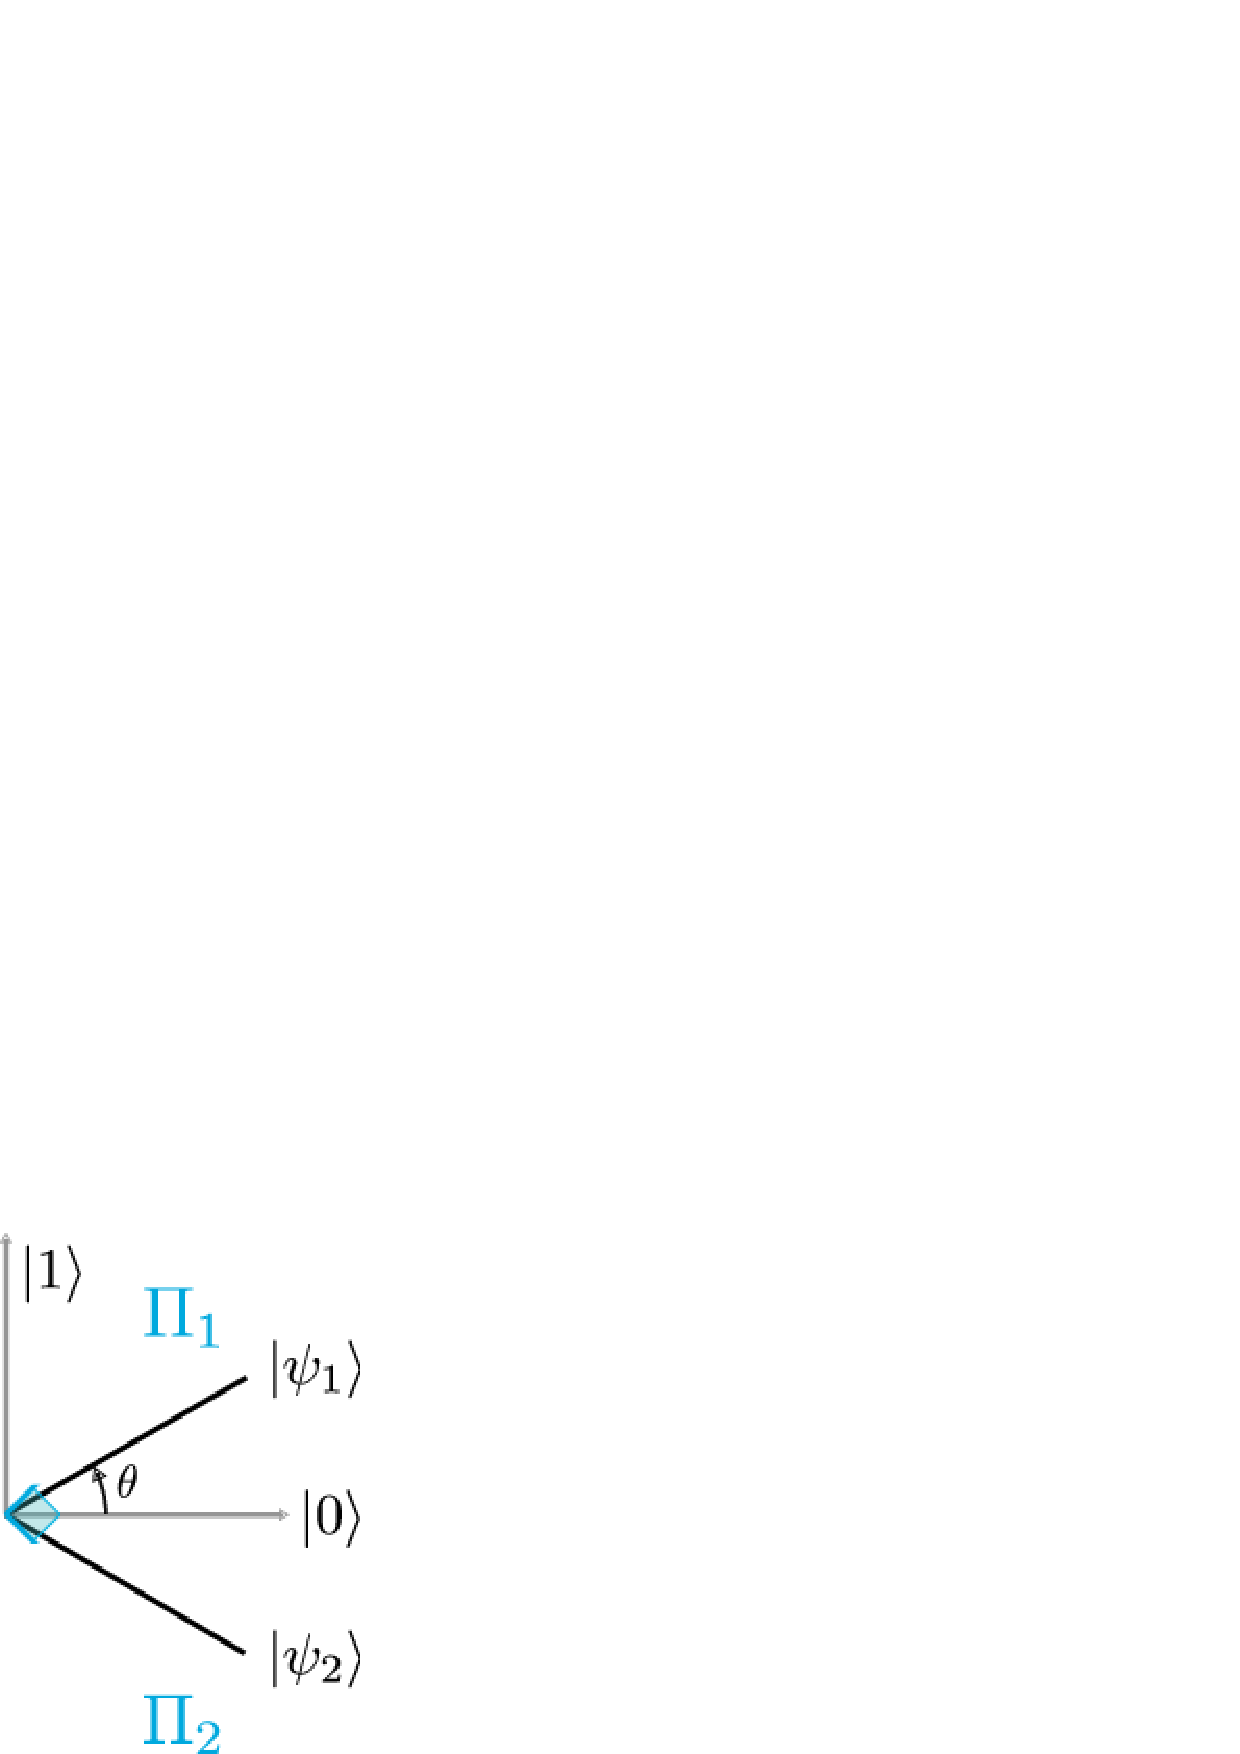
\includegraphics[height=7 cm]{ME.png} \\

\end{array}%
$%
$
\begin{figure}[th]
\centering
%
\begin{array}{c}
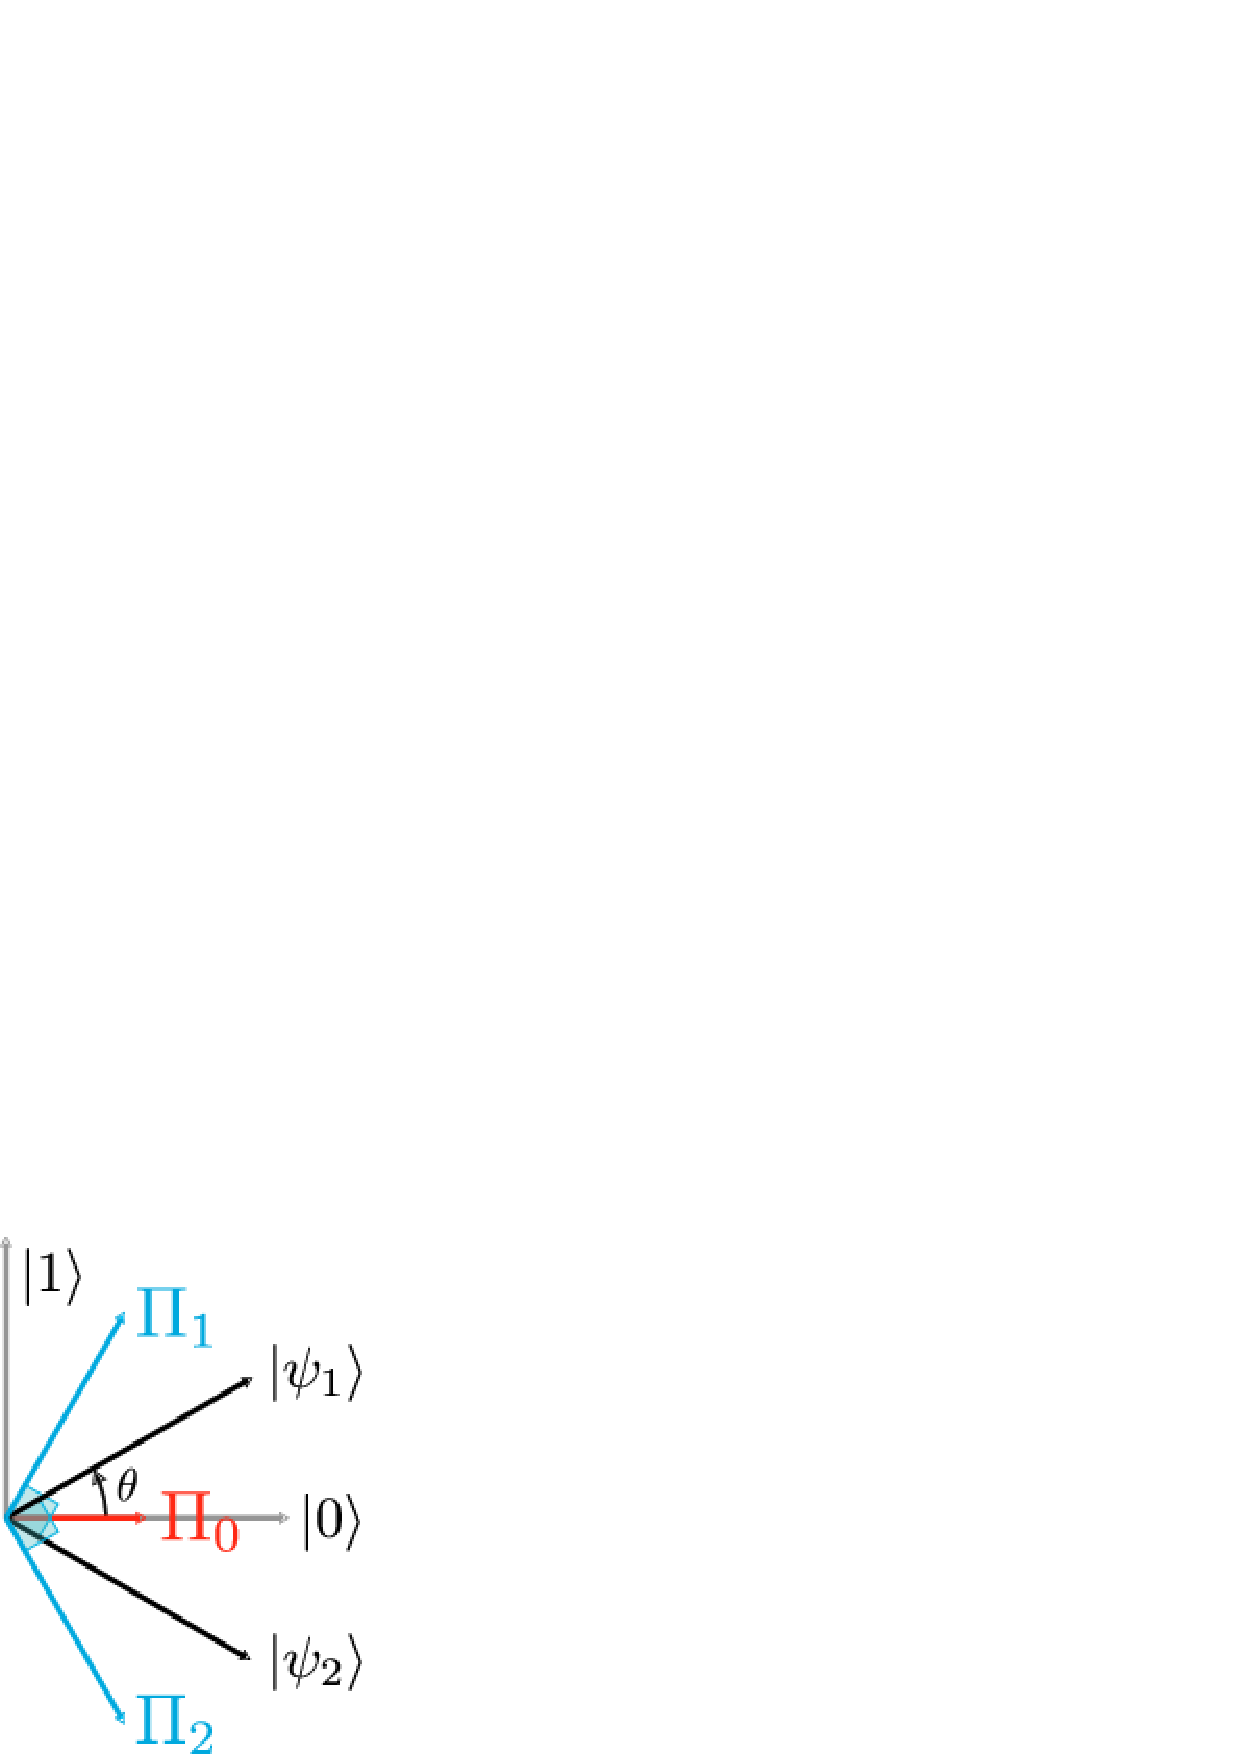
\includegraphics[height=7 cm]{UD.png} \\

\end{array}%
\end{figure}
$%

\begin{figure}[h]
\centering
$%
\begin{array}{c}
\includegraphics[height=4 cm]{Figure3.png} \\

\end{array}%
$%
\caption{Q vs Qi for all iterations with $Q_3$, $Q_1$, $Q_2$ from top to bottom}
\label{fig:Graphs}
\end{figure}

e}[th]
\centering
$%
\begin{array}{c}
\includegraphics[height=4 cm]{GraphOfRoot.jpg} \\ 
\mbox{(a)} \\ 

\end{array}%
$%
\caption{(a) $p_R$, the root of c, as a function of $0 \leq \sin^2 \theta \leq 1$ and $\frac{1}{2} \leq \eta_1 \leq 1$}
\end{figure}
